\chapter{Multilateración basada en WiFi}




\section{Simulación}





\begin{figure}[!htb]
	\centering
	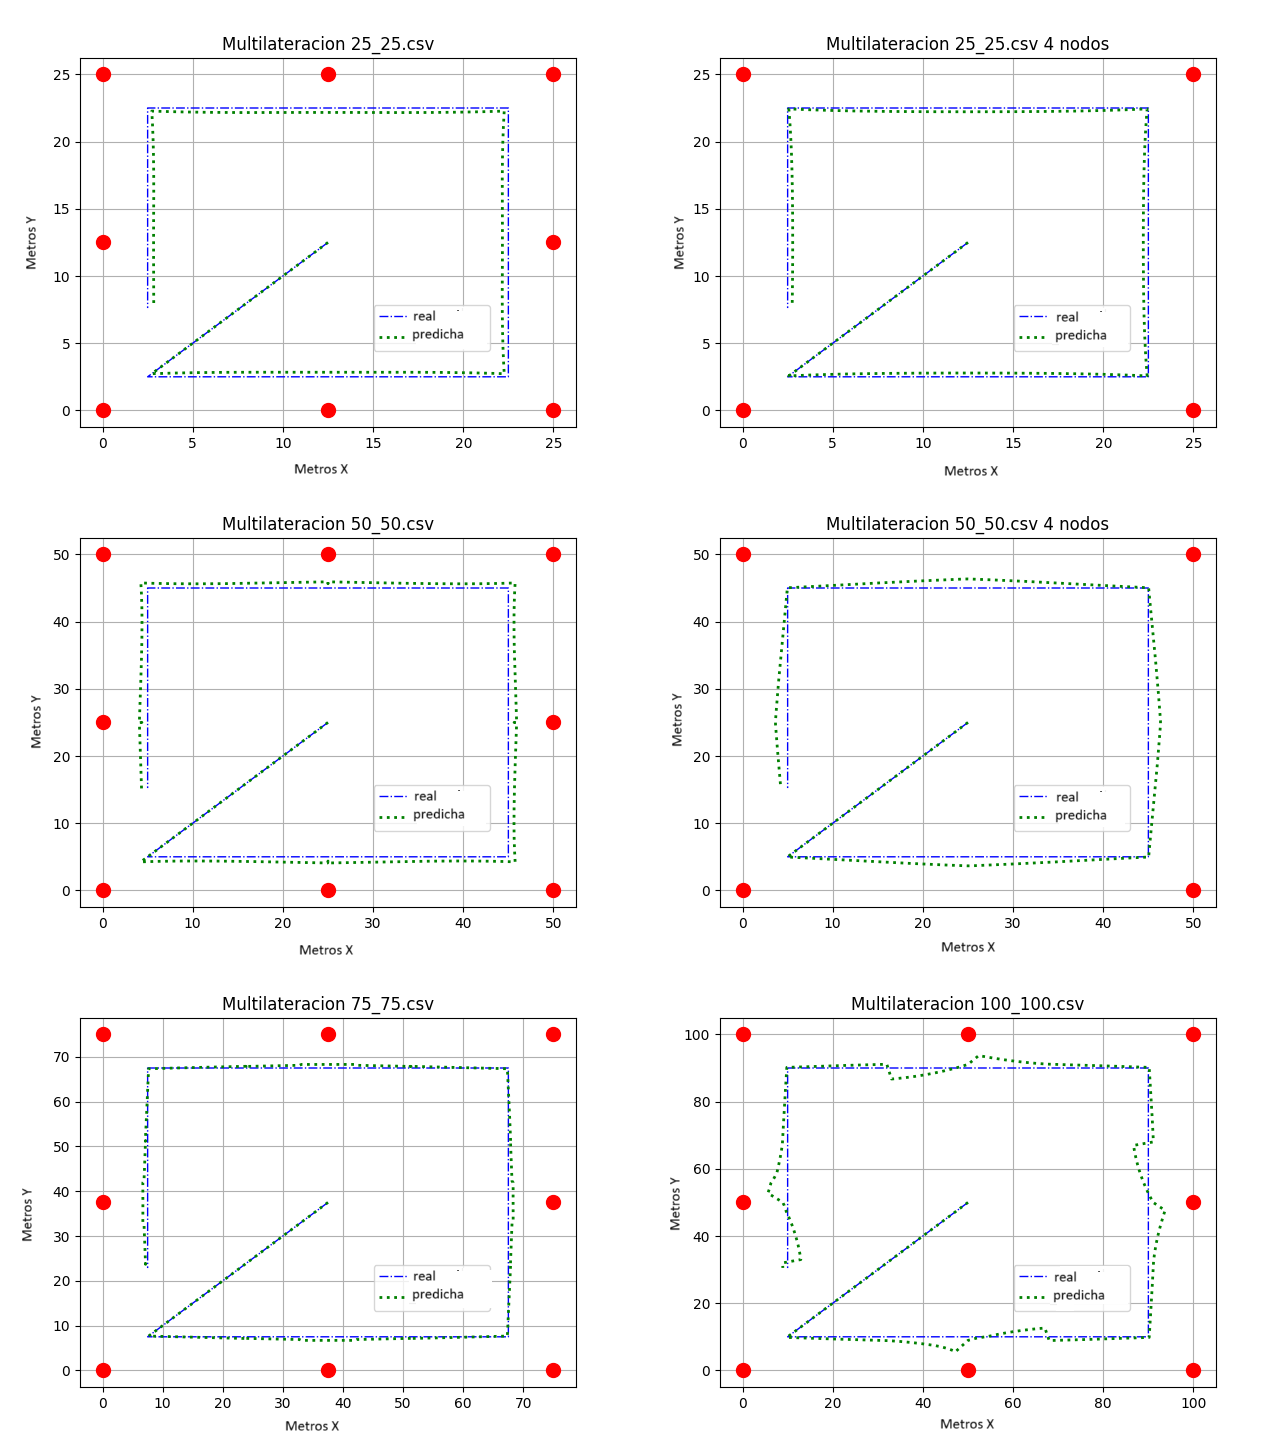
\includegraphics[width=0.8\textwidth]{Figuras/multilateration/simulated/many-sizes-and-node-count.png}
	\captionsetup{margin=2cm}
	\caption[Multilateración simulada]{Multilateración simulada, se toman los datos de la simulación en NS3 mas el N y A hallados y podemos conseguir ubicar a los nodos con los paquetes capturados.}
	\label{fig:infra-diagram}
\end{figure}

\section{Experimento Real}





Los resultados de la multilateración se compararon con la trayectoria conocida del nodo \textbf{Objetivo} para evaluar la precisión del método. Los resultados indicaron un cierto grado de error en la estimación de la ubicación, que se discutirá en la siguiente sección.


Los resultados de la multilateración, en la figura \ref{fig:real-multilateration} y \ref{fig:real-multilateration-results} se pueden observar junto a su comparación con la trayectoria conocida del nodo \textbf{Objetivo} para evaluar la precisión del método. En el gráfico, los nodos \textbf{Sniffer} se ubican en posiciones fijas, mientras que el nodo \textbf{Objetivo} se mueve a lo largo de una trayectoria conocida.

Cada punto en el gráfico representa una estimación de la ubicación del nodo \textbf{Objetivo}, calculada utilizando las mediciones de \textit{RSSI} de varios nodos \textbf{Sniffer}, el número de secuencia de paquetes y los parámetros \textbf{A} y \textbf{N} obtenidos de los experimentos de perfilado.

La línea azul representa la trayectoria real del nodo \textbf{Objetivo}, mientras que la linea verde representa las estimaciones de la ubicación del nodo \textbf{Objetivo} obtenidas a través de la multilateración. Puede observarse que las estimaciones de ubicación tienden a formar una figura similar al recorrido original pero con deformaciones.

A medida que el nodo \textbf{Objetivo} se mueve a través del área de cobertura de los \textbf{Sniffer}, hay algunas áreas en las que las estimaciones se desvían de la trayectoria real. Estas desviaciones pueden deberse a factores tales como interferencia inalámbrica, rotación involuntaria del nodo \textbf{Objetivo} mientras se lo desplaza por el recorrido, o errores en la medición del \textit{RSSI}.


\begin{figure}[!htb]
\centering
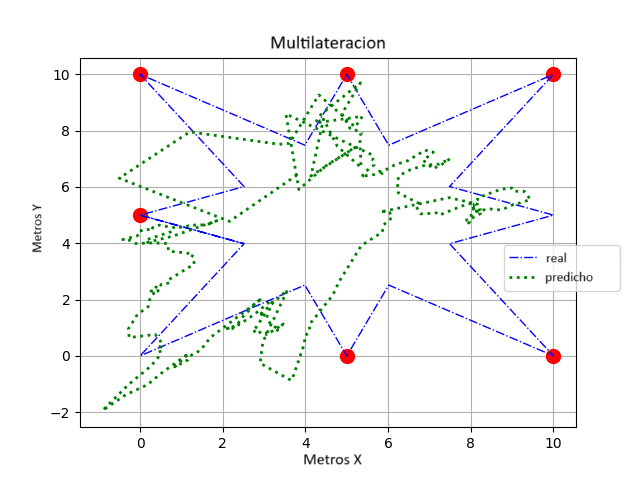
\includegraphics[width=0.8\textwidth]{Figuras/multilateration/multilateration_star.png}
\captionsetup{margin=2cm}
\caption[Configuración de la Multilateración en Tiempo Real]{Configuración del experimento de multilateración en tiempo real en el campo de deportes de la UNGS.}
\label{fig:real-multilateration}
\end{figure}

\begin{figure}[!htb]
\centering
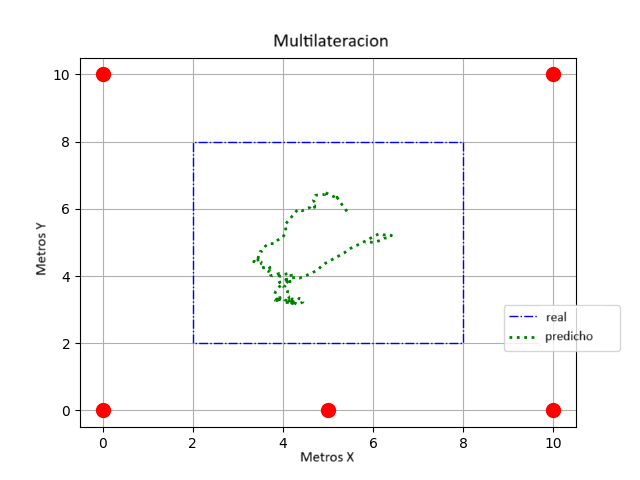
\includegraphics[width=0.8\textwidth]{Figuras/multilateration/multilateration_square.png}
\captionsetup{margin=2cm}
\caption[Resultados de la Multilateración en Tiempo Real]{Resultados de la multilateración en tiempo real, mostrando la trayectoria estimada del nodo Objetivo en comparación con su trayectoria real.}
\label{fig:real-multilateration-results}
\end{figure}